\subsection{ENVELOPING ALGEBRA OF L(X)}

THEOREM 1. Let \(\alpha: \mathrm{L}(\mathrm{X}) \to \mathrm{A}(\mathrm{X})\) be the unique Lie algebra homomorphism extending the canonical injection of \(\mathbf{X}\) into \(\mathrm{A}(\mathrm{X})\) (§ 2, no. 2, Proposition 1). Let \(\sigma \colon \mathrm{L}(\mathrm{X}) \to \mathrm{U}(\mathrm{L}(\mathrm{X}))\) be the canonical mapping of \(\mathrm{L}(\mathrm{X})\) into its enveloping algebra and let \(\beta \colon \mathrm{U}(\mathrm{L}(\mathrm{X})) \to \mathrm{A}(\mathrm{X})\) be the unique unital algebra homomorphism such that \(\beta \circ \sigma = \alpha\) (Chapter I, §2, no. 1, Proposition 1). Then:

\begin{enumerate}
\def\labelenumi{(\alph{enumi})}
\item
  \(\alpha\) is injective and \(\alpha(\mathbf{L}(\mathbf{X}))\) is a direct factor submodule of \(\mathbf{A}(\mathbf{X})\) .
\item
  \(\beta\) is bijective.
\end{enumerate}

Let B be a unital K-algebra and \(\phi\) a mapping of X into B; by Proposition 1 of §2, no. 2, there exists a Lie algebra homomorphism \(\psi\colon\mathrm{L}(\mathrm{X})\to\mathrm{B}\) such that \(\psi\mid X=\phi\) ; by Proposition 1 of Chapter I, §2, no. 1, there exists a unital algebra homomorphism \(\theta\colon\mathrm{U}(\mathrm{L}(\mathrm{X}))\to\mathrm{B}\) such that \(\theta\circ\sigma=\psi\) and hence such that \((\theta\circ\sigma)\mid X=\phi\) . As \(\sigma(\mathbf{X})\) generates the unital algebra \(\mathrm{U}(\mathrm{L}(\mathbf{X}))\) , the homomorphism \(\theta\) is the unique unital algebra homomorphism satisfying the latter condition. This shows that the ordered pair \((\mathrm{U}(\mathrm{L}(\mathbf{X}))\) , \(\sigma\mid X)\) is a solution of the same universal mapping problem as \(\mathrm{A}(\mathrm{X})\) ; taking \(\phi\) to be the canonical injection of X into \(\mathrm{A}(\mathrm{X})\) , we deduce that \(\beta\) is an isomorphism, which proves (b).

Finally, as \(\mathrm{L}(\mathrm{X})\) is a free K-module (§2, no. 11, Corollary to Theorem 1), \(\sigma\) is injective and \(\sigma(\mathrm{L}(\mathrm{X}))\) is a direct factor submodule of \(\mathrm{U}(\mathrm{L}(\mathrm{X}))\) (Chapter I, §2, no. 7, Corollary 3 to Theorem 1). By (b), this proves (a).

COROLLARY 1. There exists on the algebra \(\mathrm{A}(\mathrm{X})\) a unique coproduct making \(\mathrm{A}(\mathrm{X})\) into a bigebra such that the elements of \(\mathbf{X}\) are primitive. Further, \(\beta\) is an isomorphism of the bigebra \(\mathrm{U}(\mathrm{L}(\mathrm{X}))\) onto \(\mathrm{A}(\mathrm{X})\) with this bigebra structure.

This follows from assertion (b) of the theorem and the fact that \(\mathbf{X}\) generates the unital algebra \(\mathrm{A}(\mathbf{X})\) .

Henceforth A(X) is given this bigebra structure and L(X) is identified with its image under \(\alpha\) , that is with the Lie subalgebra of A(X) generated by X.

COROLLARY 2. If \(\mathbf{K}\) is a field of characteristic 0, \(\mathrm{L}(\mathrm{X})\) is the Lie algebra of primitive elements of \(\mathrm{A}(\mathrm{X})\) .

This follows from Corollary 1 and the Corollary to Proposition 9 of § 1, no. 5.

Remarks. (1) Let \(\mathbf{K}'\) be a commutative ring containing \(\mathbf{K}\) . If \(\mathrm{A}(\mathbf{X})\) , \(\mathrm{L}(\mathbf{X})\) and \(\mathrm{L}_{\mathbf{K}'}(\mathbf{X})\) are identified with subsets of \(\mathrm{A}_{\mathbf{K}'}(\mathbf{X})\) , we deduce from part (a) of Theorem 1 the relation

\[
\mathrm{L} (\mathrm{X}) = \mathrm{L} _ {\mathrm{K} ^ {\prime}} (\mathrm{X}) \cap \mathrm{A} (\mathrm{X}).\tag{1}
\]

\begin{enumerate}
\def\labelenumi{(\arabic{enumi})}
\setcounter{enumi}{1}
\item
  Corollary 2 to Theorem 1 remains valid if it only assumes that the additive group of the ring \(\mathbf{K}\) is torsion-free. For suppose first that \(\mathbf{K} = \mathbf{Z}\) ; every primitive element of \(\mathrm{A}(\mathbf{X})\) is a primitive element of \(\mathrm{A}_{\mathbf{Q}}(\mathbf{X})\) and hence is in \(\mathrm{L}_{\mathbf{Q}}(\mathbf{X}) \cap \mathrm{A}(\mathbf{X}) = \mathrm{L}(\mathbf{X})\) (Corollary 2 and formula (1)). In the general case, \(\mathbf{K}\) is flat over \(\mathbf{Z}\) and we apply Remark 2 of § 1, no. 2 and Proposition 3 of § 2, no. 5.
\item
  Let \(\Delta\) be a commutative monoid, \(\phi_0\) a mapping of \(\mathbf{X}\) into \(\Delta\) and \(\phi \colon \mathrm{Mo}(\mathrm{X})\to \Delta\) the homomorphism of the associated monoid; if \(\mathrm{A}(\mathrm{X})\) is given the graduation \((\mathrm{A}^{\delta}(\mathrm{X}))_{\delta \in \Delta}\) defined in Algebra, Chapter III, § 3, no. 1, Example 3 and \(\mathrm{L}(\mathrm{X})\) the graduation \((\mathrm{L}^{\delta}(\mathrm{X}))_{\delta \in \Delta}\) defined in § 2, no. 6, we have immediately, for \(\delta \in \Delta\) , \(\mathrm{L}^{\delta}(\mathrm{X})\subset \mathrm{L}(\mathrm{X})\cap \mathrm{A}^{\delta}(\mathrm{X})\) . As \(\mathrm{L}\) is the sum of the \(\mathrm{L}^{\delta}(\mathrm{X})\) for \(\delta \in \Delta\) , and the sum of the \(\mathrm{L}(\mathrm{X})\cap \mathrm{A}^{\delta}(\mathrm{X})\) for \(\delta \in \Delta\) is direct, this implies
\end{enumerate}

\[
\mathrm{L} ^ {\delta} (\mathrm{X}) = \mathrm{L} (\mathrm{X}) \cap \mathrm{A} ^ {\delta} (\mathrm{X}).\tag{2}
\]

\begin{enumerate}
\def\labelenumi{(\arabic{enumi})}
\setcounter{enumi}{3}
\tightlist
\item
  Let \(\mathbf{A}\) be a unital associative algebra and \(t = (t_i)_{i \in I}\) a family of elements of \(\mathbf{A}\) . We have a diagram
\end{enumerate}

\pandocbounded{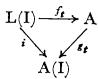
\includegraphics[keepaspectratio]{images/part001_16682a88.jpg}}

where \(i\) is the canonical injection, \(f_{t}\) is the Lie algebra homomorphism defined by \(\pmb{t}\) and \(g_{t}\) is the unital algebra homomorphism such that \(g_{t}(i) = t_{i}\) for \(i\in I\) . The diagram is commutative for \(g_{t}\circ i\) and \(f_{t}\) coincide on I. It follows that if \(\mathrm{P}\in \mathrm{L}(\mathrm{I})\) , the element \(\mathrm{P}((t_i)_{i\in I})\) defined in §2, no. 4, coincides with the element \(\mathrm{P}((t_i)_{i\in I})\) defined in Algebra, Chapter III, §2, no. 8, Example 2.

